\documentclass{standalone}
\usepackage{tikz}
\usepackage{ctex,siunitx}
\setCJKmainfont{Noto Serif CJK SC}
\usepackage{tkz-euclide}
\usepackage{amsmath}
\usetikzlibrary{patterns, calc}
\usetikzlibrary {decorations.pathmorphing, decorations.pathreplacing, decorations.shapes,}
\begin{document}
\small
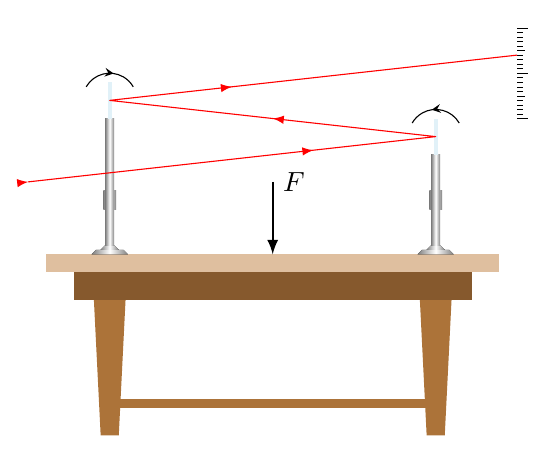
\begin{tikzpicture}[>=latex,scale=1.15]
  % \useasboundingbox(-1,-0.75)rectangle(3.7,1.4);
  \fill[brown!90!black](-2.0,0)--(-1.9,-2.0)--(-1.7,-2.0)--(-1.6,0);
  \fill[brown!90!black](2.0,0)--(1.9,-2.0)--(1.7,-2.0)--(1.6,0);
  \fill[brown!90!black](1.8,-1.7)rectangle(-1.8,-1.6);
  \fill[brown!50](-2.5,0)rectangle(2.5,-0.2);
  \fill[brown!70!black](-2.2,-0.5)rectangle(2.2,-0.2);
  \foreach \x/\y in {1.8/1.1,-1.8/1.5}
  {
    \fill[left color=gray,right color=gray,middle color=white]
    (\x+0.2,0)--(\x-0.2,0)--++(0.05,0.05)--++(0.3,0)--cycle;
    \fill[left color=gray,right color=gray,middle color=white]
    (\x+0.1,0.05)--(\x-0.1,0.05)--++(0.05,0.05)--++(0.1,0)--cycle;
    \fill[left color=gray,right color=gray,middle color=white]
    (\x+0.07,0.5)rectangle(\x-0.07,0.7);
    \fill[left color=gray,right color=gray,middle color=white](\x-0.05,0.1)rectangle(\x+0.05,\y);
    \fill[cyan!50!lightgray!20](\x-0.02,\y)rectangle(\x+0.02,\y+0.4);
  }
  \draw[thin,postaction={decorate},decoration={markings,mark=at position .57
  with {\arrow{stealth}}}]([shift=(150:0.3)]-1.8,1.7)arc(150:30:0.3);
  \draw[thin,postaction={decorate},decoration={markings,mark=at position .57
  with {\arrow{stealth}}}]([shift=(30:0.3)]1.8,1.3)arc(30:150:0.3);
  \foreach \x in {2.0,2.5}
  {
    \draw[very thin] (2.7,\x)--++(0.12,0);
    \foreach \y in {1,2,3,4,6,7,8,9}
    {
      \draw[very thin] (2.7,\x-0.05*\y)--++(0.06,0);
    }
    \draw[very thin] (2.7,\x-0.25)--++(0.09,0);
  }
  \draw[very thin] (2.7,1.5)--++(0.12,0);
  \draw[thin,red,line join=round,postaction={decorate},decoration={markings,mark=between positions 0 and 0.9 step 0.25 
  with {\arrow{>}}}](-2.7,0.8)--(1.8,1.3)--(-1.8,1.7)--(2.7,2.2);
  \draw[thick,->](0,0.8)--(0,0)node[at start,right]{$F$};
  \end{tikzpicture}
\end{document}